\documentclass[8pt,xcolor={usenames,dvipsnames}]{beamer}
\setbeamercovered{transparent}
\usepackage[utf8]{inputenc}
\usepackage[english]{babel}
\usetheme{Warsaw}
\usecolortheme{fly}
\geometry{paperwidth=140mm,paperheight=105mm}
\usepackage{minted}
\usemintedstyle{monokai}
\usepackage{tikz}
\usepackage{verbatim}
\usetikzlibrary{arrows,shapes}

\begin{document}
\definecolor{darkolive}{RGB}{3,17,7}
\setbeamercolor{author}{fg=SkyBlue}
\setbeamercolor{date}{fg=white}
\title{Django, reportes e impresión}
\author{Igor Támara}
\date{Diciembre 4 de 2014}

\setbeamercolor{normal text}{fg=white,bg=darkolive}
\setbeamercolor{structure}{fg=white}
\setbeamercolor{abstract}{fg=white}
\setbeamercolor{abstract title}{fg=white}

\setbeamercolor{alerted text}{fg=red!85!black}

\setbeamercolor{item projected}{use=item,fg=white,bg=darkolive}

\setbeamertemplate{enumerate items}[default]
\setbeamertemplate{navigation symbols}{}
\setbeamercovered{transparent}
\setbeamercolor*{item}{fg=white,bg=darkolive}
\setbeamercolor*{item projected}{fg=white,bg=darkolive}
\setbeamercolor*{itemize item}{fg=white,bg=darkolive}
\setbeamercolor*{itemize subitem}{fg=white,bg=darkolive}
\setbeamercolor*{itemize subsubitem}{fg=white,bg=darkolive}
\setbeamercolor*{itemize/enumerate body}{fg=white,bg=darkolive}
\setbeamercolor*{itemize/enumerate subbody}{fg=white,bg=darkolive}
\setbeamercolor*{itemize/enumerate subsubbody}{fg=white,bg=darkolive}
\setbeamercolor*{palette primary}{use=structure,fg=structure.fg}
\setbeamercolor*{palette secondary}{use=structure,fg=structure.fg!95!black}
\setbeamercolor*{palette tertiary}{use=structure,fg=structure.fg!90!black}
\setbeamercolor*{palette quaternary}{use=structure,fg=structure.fg!95!black,bg=black!80}
\setbeamercolor*{section in toc}{fg=white,bg=darkolive}
\setbeamercolor*{subsection in toc}{fg=white,bg=darkolive}
\setbeamercolor*{subsubsection in toc}{fg=white,bg=darkolive}
\setbeamercolor*{framesubtitle}{fg=white}

\setbeamercolor*{block title}{parent=structure,bg=black!60}
\setbeamercolor*{block body}{fg=white,bg=black!10}
\setbeamercolor*{example text}{fg=white,bg=black!10}
\setbeamercolor*{verse}{fg=white,bg=black!10}
\setbeamercolor*{quotation}{fg=white,bg=black!10}
\setbeamercolor*{quote}{fg=white,bg=black!10}
\setbeamercolor*{block title alerted}{parent=alerted text,bg=black!15}
\setbeamercolor*{block title example}{parent=example text,bg=black!15}

\frame{\titlepage} 

\section{Ruta}

\subsection{Printing Time!!!!}

\frame{\frametitle{Table of contents}\tableofcontents} 


\begin{frame}
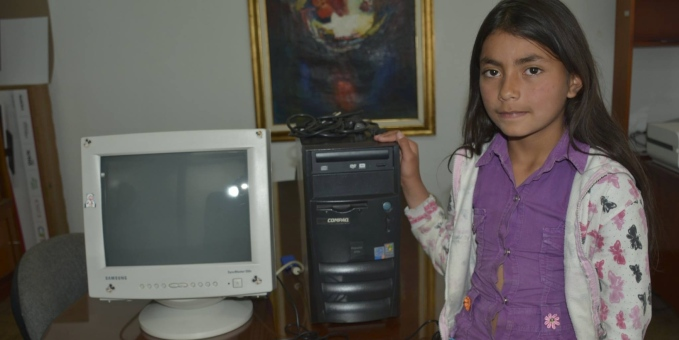
\includegraphics[width=\paperwidth]{images/kemosion.jpg}

\end{frame}

\section{Algunas Opciones}

\subsection{Formatos preimpresos}

\begin{frame}[fragile]
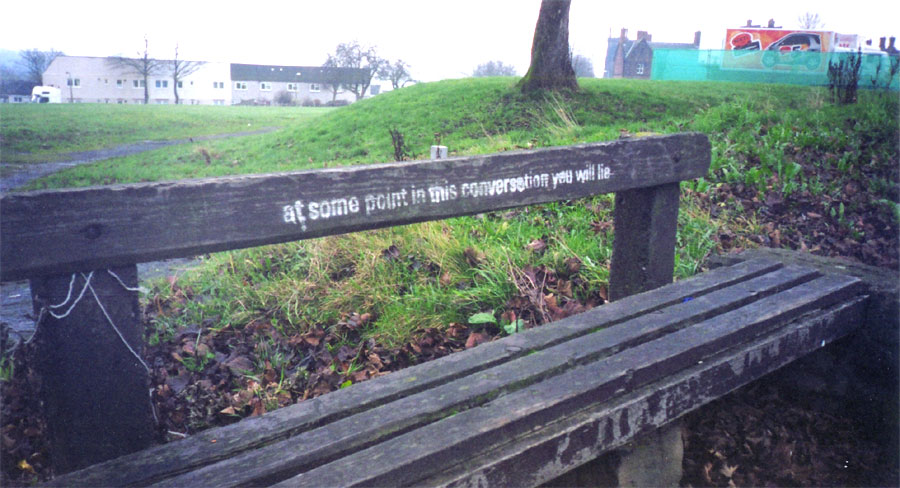
\includegraphics[width=\paperwidth]{images/graffiti.jpg}

\end{frame}


\begin{frame}[fragile]
\frametitle{pdfrw}
\begin{minted}{python}
from cStringIO import StringIO
from pdfrw import PdfReader

filein = PdfReader('/tmp/myfile') # PDF Base

...

canvas.drawString(3800, height - 300, unicode('Hola Mundo'))

canvas.showPage()
canvas.save()
pdf = pdf_buffer.getvalue()
pdf_buffer.close()

# Un pdf con algunos textos encima
# Los trucos incluyen contar con reportlab

\end{minted}
\end{frame}

\begin{frame}
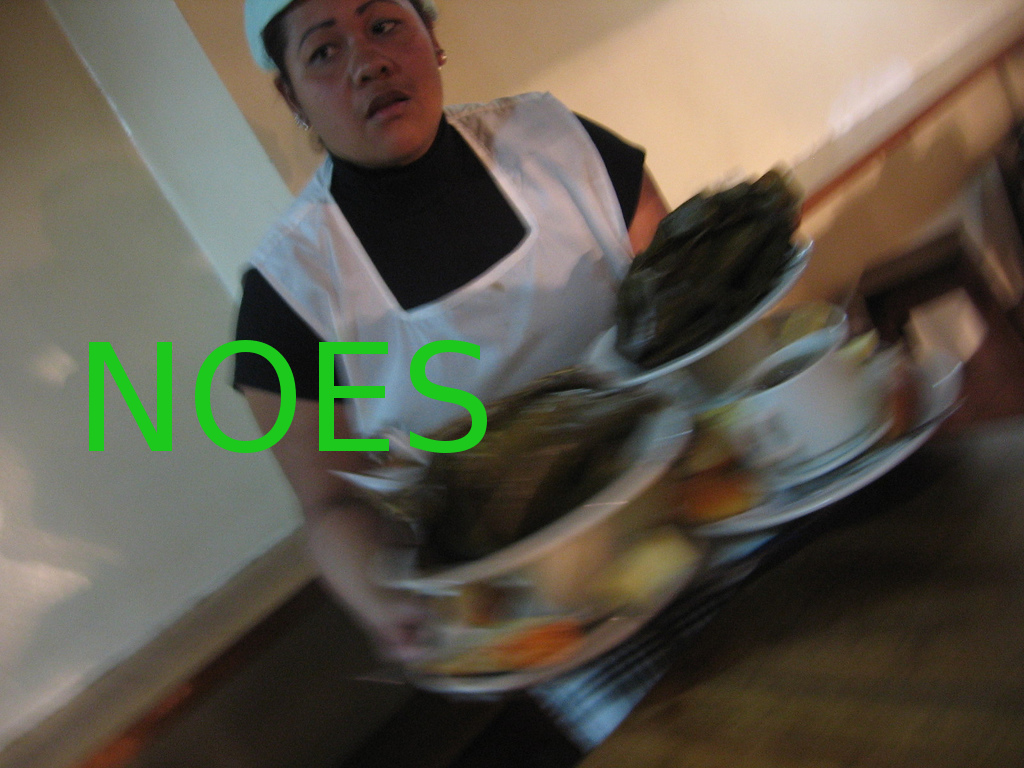
\includegraphics[width=\paperwidth]{images/noestamal.jpg}

\end{frame}

\subsection{Aprovechando capacidades del navegador}

\begin{frame}[fragile]
\frametitle{CSS}
\begin{minted}{css}
@media print {
    header nav, footer {
        display: none;
    }

...

}

/* Con su maquetador favorito y media print, no se garantiza
margen o encabezados.

Ahorra papel y evita talar
*/
\end{minted}
\end{frame}

\begin{frame}[fragile]
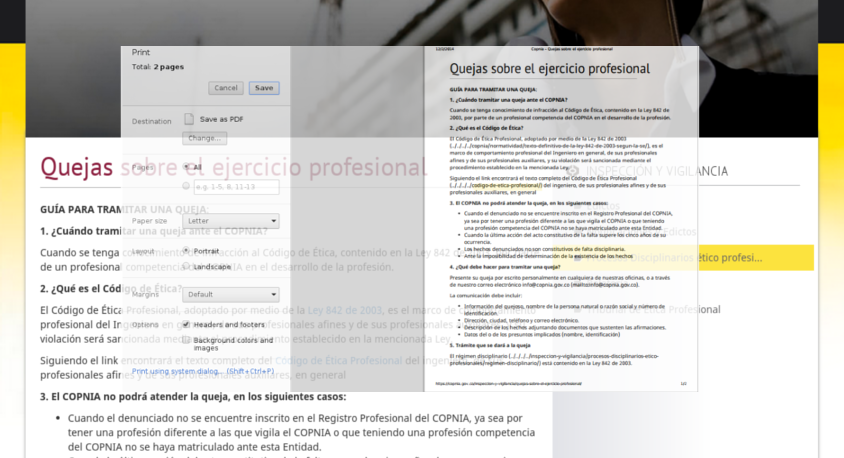
\includegraphics[width=\paperwidth]{images/cssmediaprint.png}

\end{frame}

\subsection{De html a PDF}

\begin{frame}

\includegraphics[width=\paperwidth]{images/lazydog.jpg}

\end{frame}

\subsection{\LaTeX}

\begin{frame}


\includegraphics[height=\paperheight]{images/tugboat_tfz.png}

\end{frame}

\begin{frame}
\frametitle{\LaTeX}

\tikzstyle{format} = [draw, thin, fill=blue!20]
\tikzstyle{medium} = [ellipse, draw, thin, fill=green!20, minimum height=2.5em]

\begin{figure}
\begin{tikzpicture}[node distance=3cm, auto,>=latex', thick]
    % We need to set at bounding box first. Otherwise the diagram
    % will change position for each frame.
    \path[use as bounding box] (-1,0) rectangle (10,-2);
    \path[->]<1-> node[format] (py) {.py file}
                  node[format, below of=py] (sty) {.sty file};
    \path[->]<2-> node[format, right of=py] (tex) {.tex file}
                  (py) edge[color=yellow] node {Python} (tex);
    \path[->]<3-> node[format, right of=tex] (pdf) {.pdf file}
                  (sty) edge[color=yellow] node {\LaTeX} (pdf)
                  (tex) edge[color=yellow] node {\LaTeX} (pdf)
                  node[medium, below of=pdf] (user) {User};
    \path[->]<4-> (pdf) edge[color=yellow] node {Django} (user);
\end{tikzpicture}
\end{figure}
\end{frame}

\begin{frame}[fragile]
\frametitle{Armando con \LaTeX}
\begin{minted}{python}
# Se verifica que no se haya creado el archivo,
# en tal caso se crea con algo como
...
from subprocess import call

ret = call('pdflatex -output-directory={0} {1}'.format(
    wdirectory,  # Directorio destino
    name,        # Nombre del archivo
), shell=True)

# Este archivo se sirve con los permisos correspondientes

# En nuestro caso creamos nuestra clase con variables, ambientes
# y se concatena el texto para generar el .tex

\end{minted}
\end{frame}


\section{ReportLab}

\subsection{Características}

\begin{frame}
  \frametitle{Características}
  \begin{itemize}
  \item Códigos de barras, QR
  \item Tablas
  \item Oportunidad de definir diferentes templates, portada, internas
  \item Numeración automática de páginas
  \item Sabe a python
  \item Bajo nivel
  \item Control sobre el tamaño del papel
  \item Inclusión de imágenes
  \item Definición de plantillas
  \item Hosted solution
  \item Open Source
  \item Ejemplo en documentación de Django
  \end{itemize}
\end{frame}

\subsection{python time}
  
\begin{frame}[fragile]
\frametitle{Puro y duro}
\begin{minted}{python}
from reportlab.pdfgen import canvas  
from reportlab.lib.units import cm
from reportlab.lib.units import mm
from reportlab.graphics.barcode.qr import QrCodeWidget
from reportlab.graphics.shapes import Drawing
from reportlab.graphics import renderPDF
from reportlab.lib.pagesizes import letter

c = canvas.Canvas('/tmp/hello.pdf', pagesize=letter)  
c.drawString(9*cm, 22*cm, 'Hola mundo')

# QR :) , so welcome
qrw = QrCodeWidget('http://osm.org', barWidth=32 * mm, barHeight=32 * mm)
qr_code = Drawing(31 * mm, 31 * mm)
qr_code.add(qrw)
renderPDF.draw(qr_code, c, 9*cm, 25*cm)

c.showPage()  
c.save()

\end{minted}
\end{frame}

\subsection{De nuevo html a PDF}

\begin{frame}

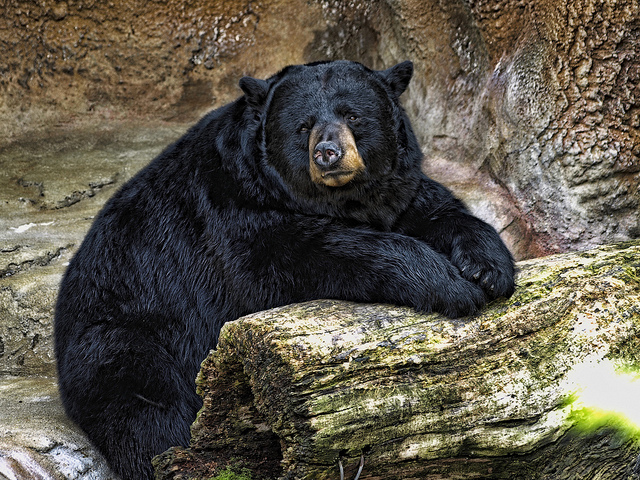
\includegraphics[height=\paperheight]{images/sleepybear.jpg}

\end{frame}

\subsection{RML}

\begin{frame}

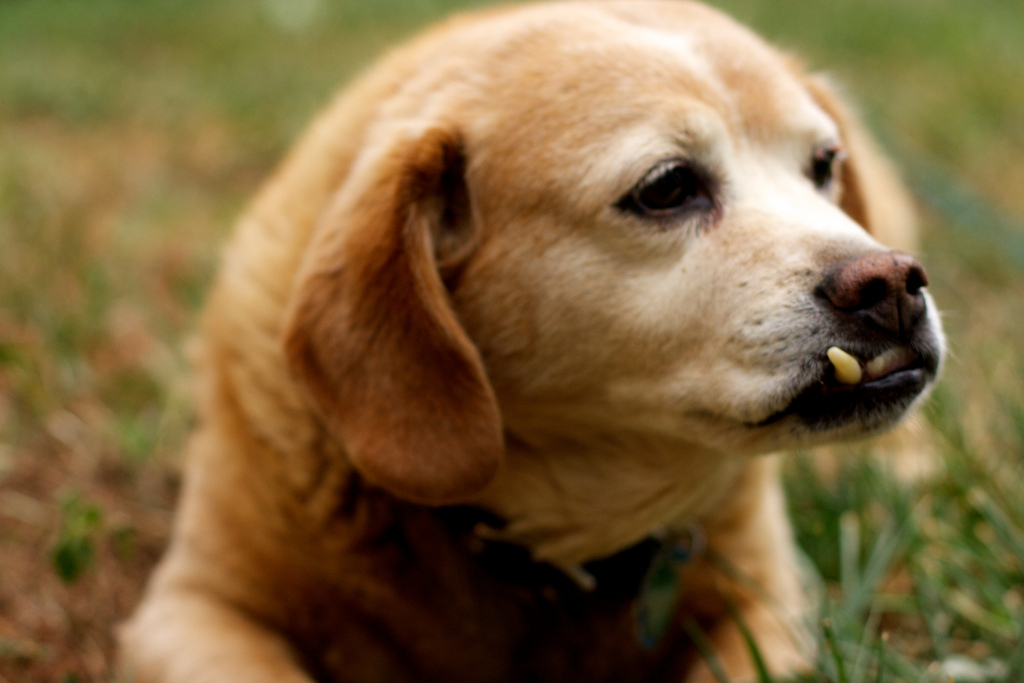
\includegraphics[width=\paperwidth]{images/uglyxml.jpg}

\end{frame}

\begin{frame}[fragile]
\frametitle{Hola mundo en RML}
\begin{minted}{xml}
<!DOCTYPE document SYSTEM "rml.dtd">
<document filename="example_1.pdf">
 <stylesheet>
 </stylesheet>
 <pageDrawing>
   <drawCentredString x="4.1in" y="5.8in">
     Hola mundo
   </drawCentredString>
   <barCode code="QR" x="4.1in" y="10.6in" >http://osm.org</barCode>
 </pageDrawing>
</document>
\end{minted}

\end{frame}

\begin{frame}
\frametitle{RML rocks}
\begin{itemize}
\item 100\pounds mensuales por uso vía reportlab
\item Buenos ejemplos
\item Flowables
\item Plantillas
\item Template / Stylesheet / Story
\item Tablas
\item Imágenes
\item Gráficas
\item 5X en productividad frente a Reportlab
\end{itemize}
\end{frame}

\subsection{z3c.rml}

\begin{frame}[fragile]
\frametitle{Usando z3c.rml}
\begin{minted}{python}
from z3c.rml import rml2pdf
...

class PdfCertificateView(View):
    the_doc = render_to_string('layout/base_certificate_pdf.rml', {...})
    pdf_doc = rml2pdf.parseString(the_doc)
    pdf_doc.seek(0)

    response = HttpResponse(content_type='application/pdf')
    response['Content-Disposition'] = u'attachment; filename=mi_cert.pdf'
    response.write(pdf_doc.read())
    return response

\end{minted}
\end{frame}

\section{Otras aproximaciones}
\subsection{wkhtmltopdf, xhtml2pdf, relatorio}

\begin{frame}
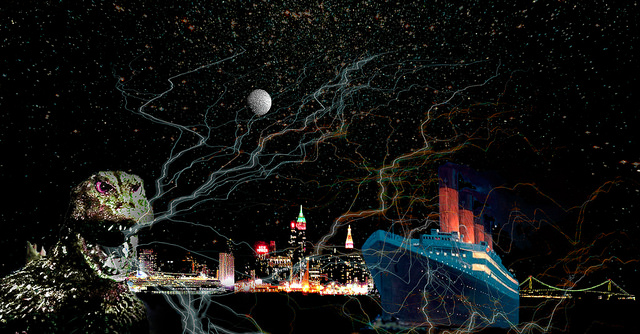
\includegraphics[width=\paperwidth]{images/loo.jpg}
\end{frame}


\begin{frame}
  \begin{itemize}
  \item wkhtmltopdf
    \begin{itemize}
      \item No se escribe nada específico para impresión
      \item Heredado de prácticas desde otros lenguajes populares
      \item Paquete de pypi
      \item wrapper para Django
      \item Lo usa la wikipedia
      \item soporte para flash
    \end{itemize}
  \item xhtml2pdf
    \begin{itemize}
    \item Estilizable vía CSS
    \item construído sobre reportlab
    \end{itemize}
  \item relatorio
    \begin{itemize}
    \item Hacer el template en .odt
    \item Hacer los reemplazos con relatorio
    \item Exportar a PDF
    \item En pypi
    \end{itemize}
  \end{itemize}

\end{frame}


\section{PQR}

\begin{frame}
\frametitle{Ack}
  \begin{itemize}
  \item Niña de Pasto Diario ADN
  \item Steven Taylor https://flic.kr/p/ckQP
  \item Natalia Vivas https://flic.kr/p/2anQ8p
  \item notinthedoghouse http://bit.ly/1vMiSCd
  \item Tex Lion fiee.net
  \item DazzlingDigitalPhotography https://flic.kr/p/7R2iQZ
  \item radloff https://flic.kr/p/8qFX95
  \item Leonardo Dell'Aquila https://flic.kr/p/5pA8Go
  \item Russ Seidel https://flic.kr/p/jPMWi8
  \item Axiacore
  \item igor@tamarapatino.org
  \item CC Share Alike, do what you want with this
  \item No warranties
  \end{itemize}
\end{frame}

\begin{frame}
\frametitle{Sin garantías}
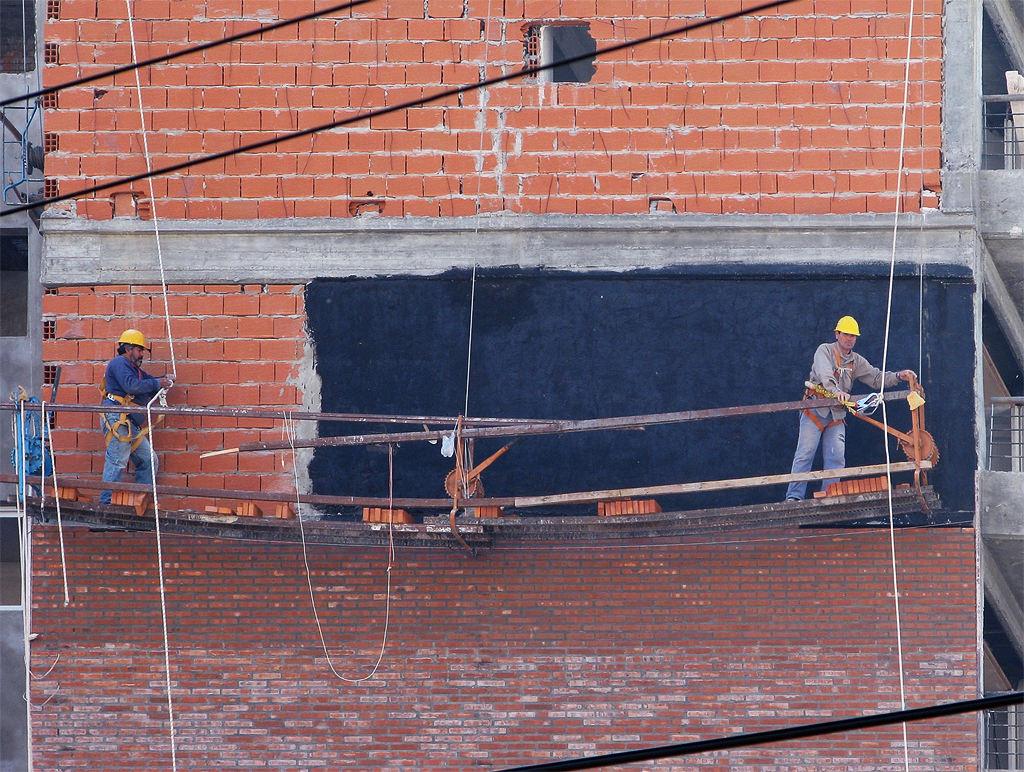
\includegraphics[height=\paperheight]{images/nowarranty.jpg}
\end{frame}

\end{document}
